\chapter{Results}
In this section we present and compare results of the six models aplied in STLF. The performance of the models are evaluated using MAPE, MAE, RMSE and $R^2$. These metrics can give us a clear picture and comparisons framework for each of the model performance.  The goal is to represent the accuracy, robustness and suitability of the ML and AI models to solve STLF.




\section{Dataset Preprocessing Results}
 The continuous\_dataset.csv contained continuous time series data. The empty slots were filled using the forward and back-filling process.Figure \ref{fig:originaldataset}
 \begin{figure}[h]
 	\centering
 \begin{minipage}[b]{0.45\linewidth}
 	\centering
 	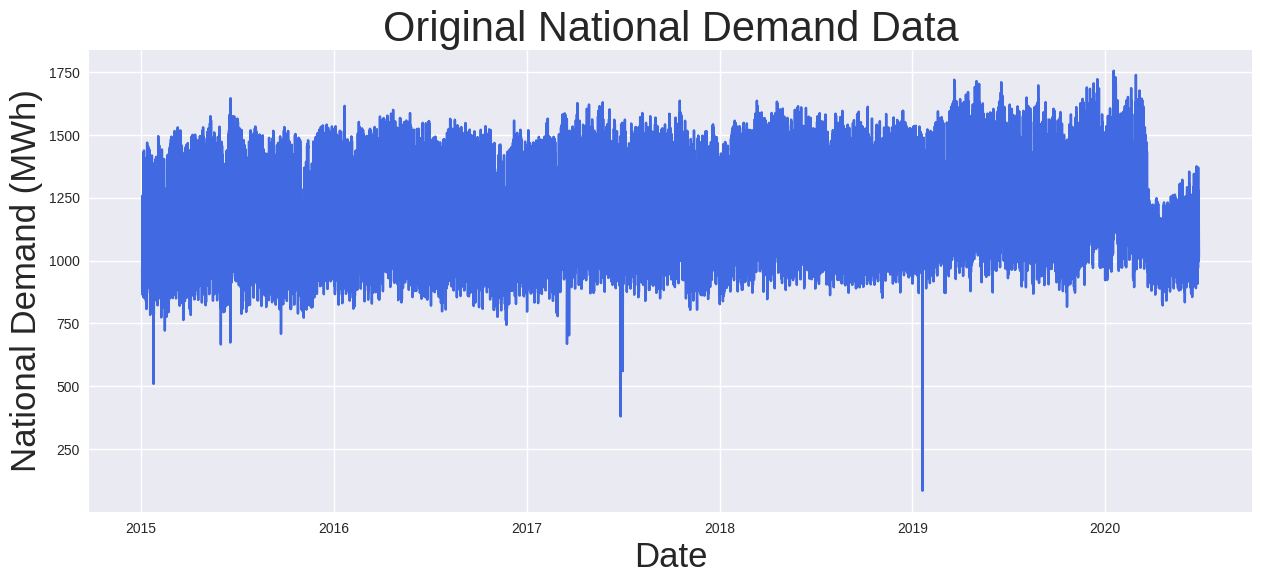
\includegraphics[width=\linewidth]{Chapters/images/results/original_dataset}
 	\caption{The original national demand .}
 	\label{fig:originaldataset}
 \end{minipage}
 \begin{minipage}[b]{0.45\linewidth}
 	\centering
 	\includegraphics[width=\linewidth]{"Chapters/images/results/train test split_after HI"}
 	\caption{HI processed dataset with traintest split.}
 	\label{fig:train-test-splitafter-hi}
 \end{minipage}
 \end{figure}
 
 The HI method explained in section \ref{sec:HI_method}, was used to handle outliers in the dataset, fixing all data-points that deviated from the normalcy.  After implementing the HI-method the train test split of 80/20 was implemented with a validation set ratio of 0.2 of the testing data. Figure \ref{fig:train-test-splitafter-hi} shows the effectiveness of the HI method in removing noisy details in the dataset.

 \begin{figure}[h]
  	\centering
  	% First figure
  	\begin{minipage}[b]{0.45\linewidth}
  		\centering
  		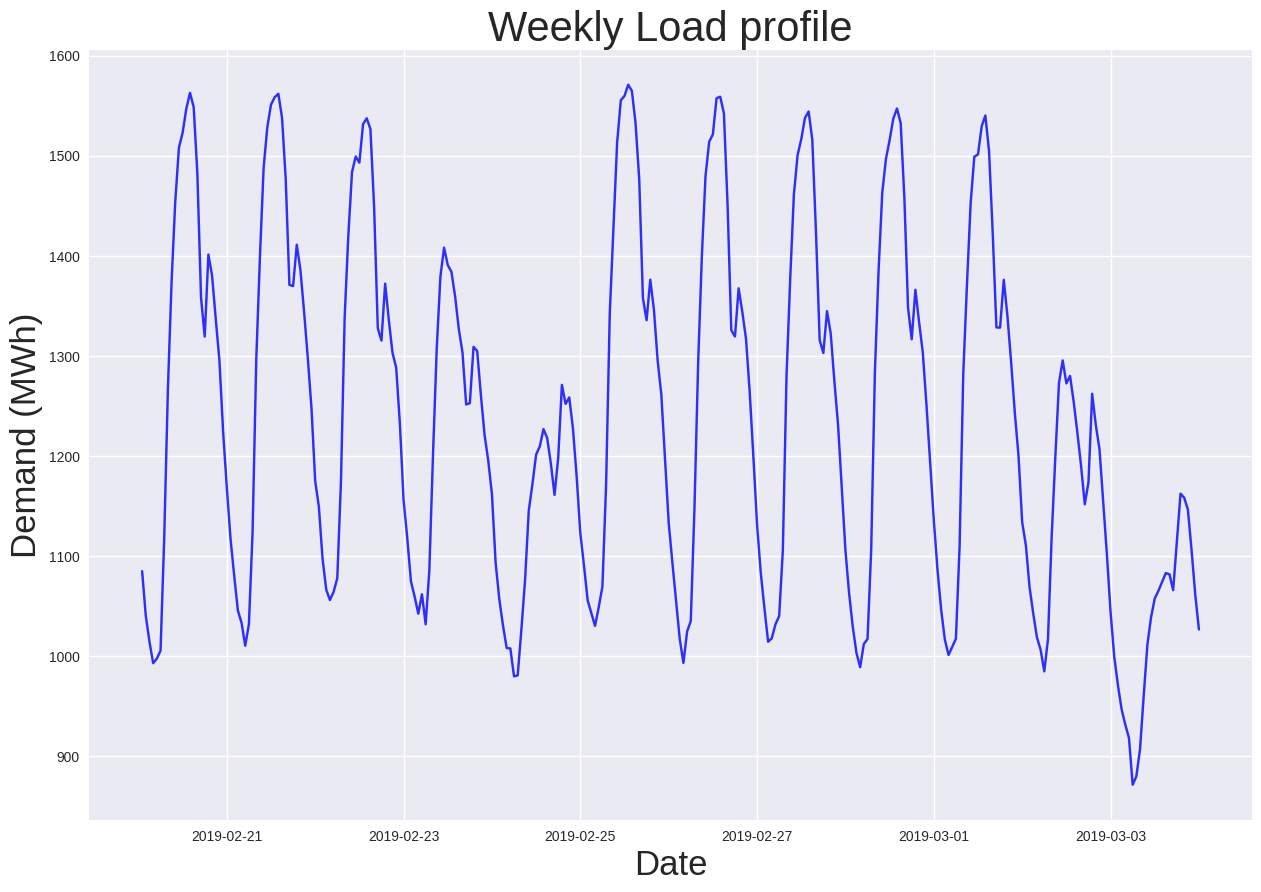
\includegraphics[width=\linewidth]{Chapters/images/results/weekly_load_profile.png}
  		\caption{The general weekly national load profile.}
  		\label{fig:weeklyloadprofile}
  	\end{minipage}
  	\hfill
  	% Second figure
  	\begin{minipage}[b]{0.45\linewidth}
  		\centering
  		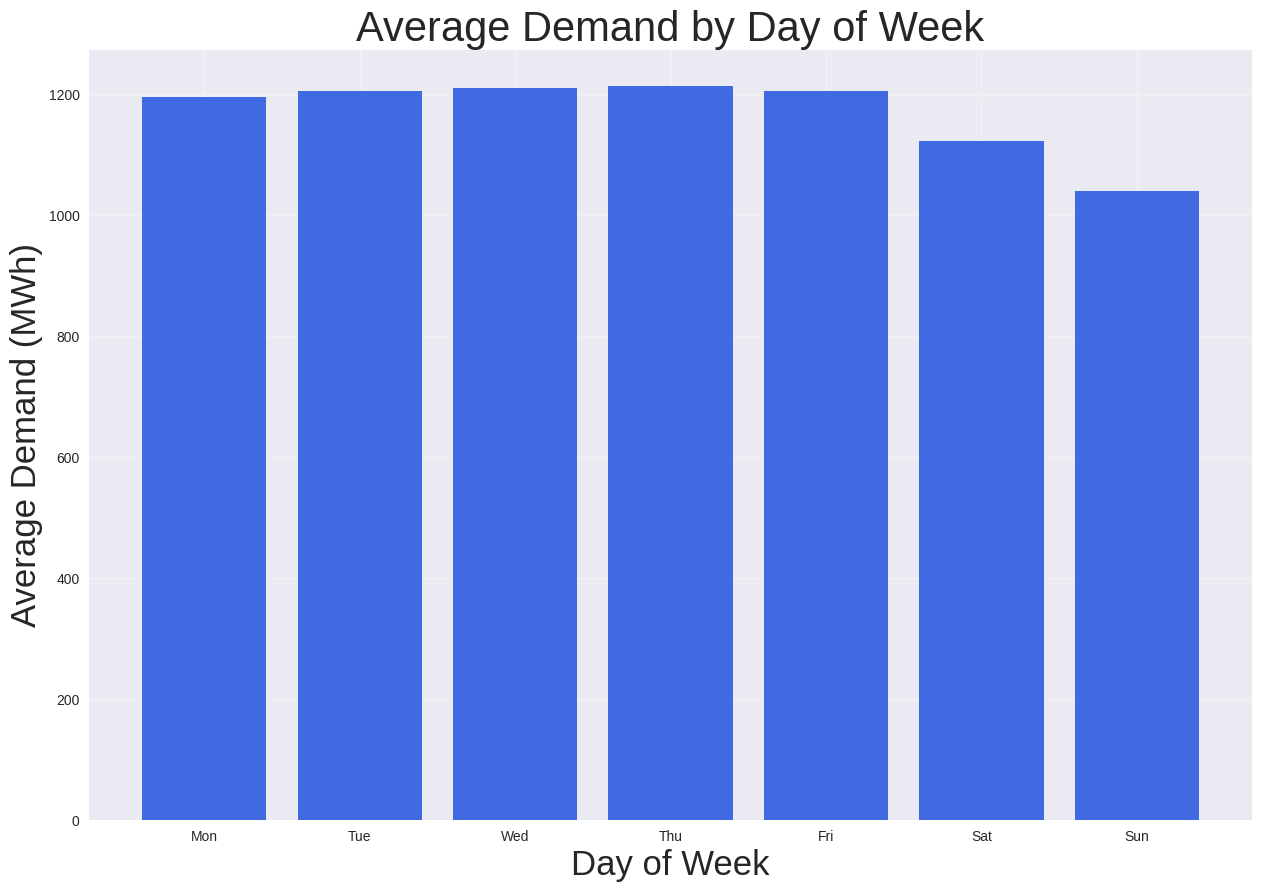
\includegraphics[width=\linewidth]{Chapters/images/results/average_daily_demand.png}
  		\caption{The weekly average daily demand }
  		\label{fig:averagedailydemand}
  	\end{minipage}
  \end{figure}
  
  
The weekly load profile in figure \ref{fig:weeklyloadprofile} shows a daily pattern that the load exhibits.The trend shows a higher usage during the week and lower usage in the weekend, with the lowest usage day being Sunday. This phenomenon represents a load profile that is found in places with industries that has maximum load requirements during the day. Figure \ref{fig:averagedailydemand} shows the average daily demand  of electricity. It also shows a higher usage during the week and lower consumption on the weekend, with Sunday being the lowest consumption day. 
  \begin{figure}[h]
  	\centering
  	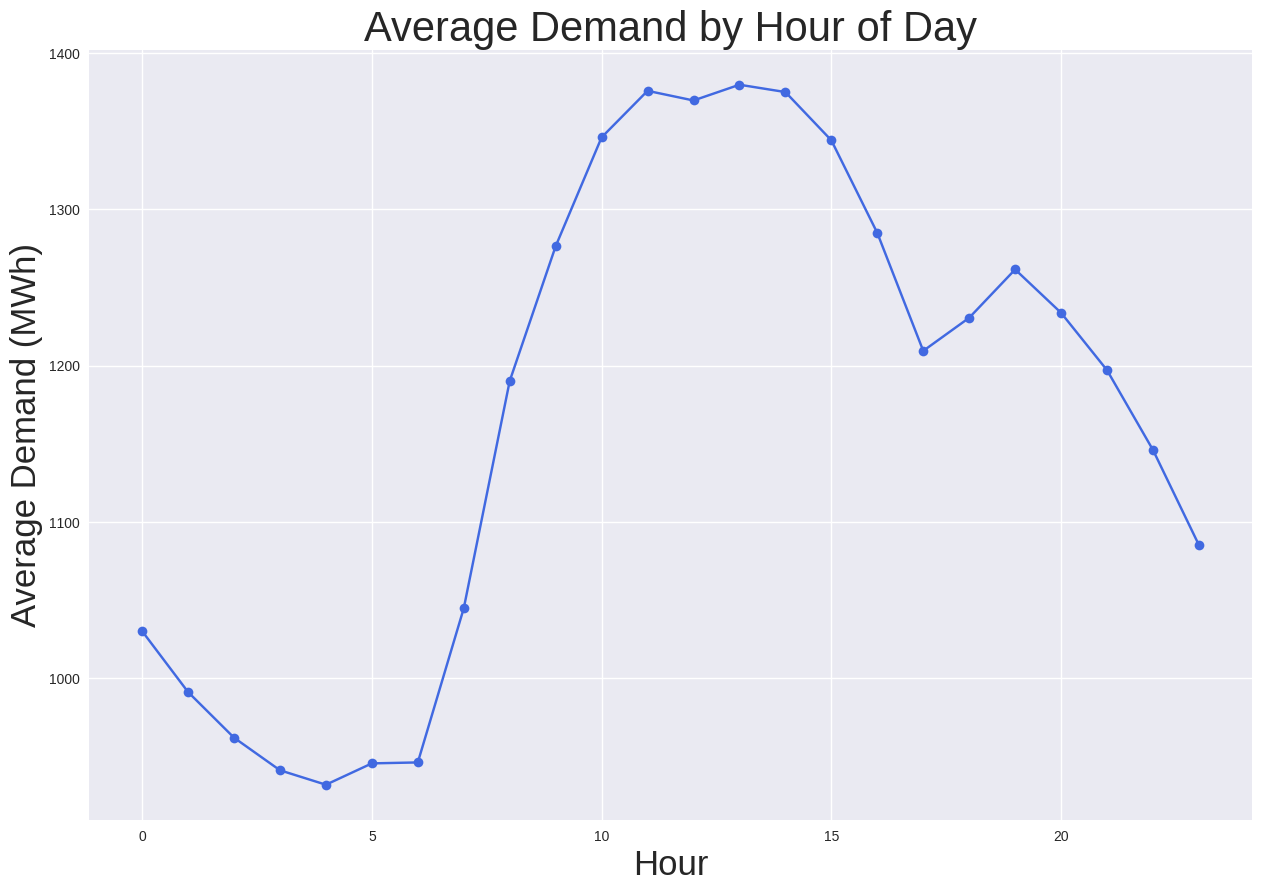
\includegraphics[width=0.45\linewidth]{Chapters/images/results/average_hourly_demand}
  	\caption{Average hourly demand of electricity between 2015 and 2020 in panama}
  	\label{fig:averagehourlydemand}
  \end{figure}
  
  Figure \ref{fig:averagehourlydemand} shows the average hourly usage of data. The averages show that the lowest consumption is in the early hours of the day, with a steady rise in the early morning leading to a peak at midday. After midday there is a steady decrease in demand with a slight increase between the 18th and 20th hour of the day, this is followed by a drop in usage leading to the early hours of the day.  


\section{Model Simulation Results}

\subsection{Exponential smoothing}
\subsubsection{Model Choice result}
The algorithm in Appendix \ref{sec:appendixA}, figure \ref{fig:exponential-smoothing-model-choice} was used to find the best model to use for the ES model. Table \ref{tab:es_model_selection} shows the ES models and a parameters that were tested to find the best model.

\begin{table}[ht]
	\centering
	\resizebox{\textwidth}{!}{%
		\begin{tabular}{lccccccc}
			\hline \\
			\textbf{Model} & \textbf{Trend} & \textbf{Seasonality} & \textbf{Seasonality Period} & \textbf{Damped} & \textbf{MAPE (\%)} & \textbf{MSE (MWh)} & \textbf{AIC}
			\\
			\hline
			Simple               & None  & None & –  & No  & 13.76\%  & 180.98 & 343990.96 \\
			Double               & Add   & None & –  & No  & 15.14\%  & 172.11 & 327001.68 \\
			Triple\_Add          & Add   & Add  & 24 & No  & 10.56\%  & 125.56 & 277981.02 \\
			Triple\_Mul          & Mul   & Mul  & 24 & No   & 34.48\%  & 408.23 & 272265.85 \\
			Triple\_Add\_Damped  & Add   & Add  & 24 & Yes &  9.99\%  & 120.81 & 277708.98 \\
			Triple\_Mul\_Damped  & Mul   & Mul  & 24 & Yes & 10.01\%  & 119.49 & 272266.18 \\
			\hline
		\end{tabular}%
	}
	\caption{Exponential Smoothing Models chosen for benchmarking and their performance (Add = Additive , Mul = Multiplicative).}
	\label{tab:es_model_selection}
\end{table}

The best performing ES model was the Triple Multiplicative Damped algorithm, which uses a seasonality period of 24 to capture daily recurring patterns. While the MAPE and MSE values for Triple\_Add\_Damped and Triple\_Mul\_Damped are very close, the lower AIC of Triple\_Mul\_Damped indicates a better overall model fit. This model was selected as the benchmark for evaluating other forecasting approaches in this study.

\subsubsection{ES model Results}
The ES model being the benchmark model achieved a MAPE of 9.57\% with a MAE of 118.14Mwh using the Triple Multiplicative Damped configuration. Table \ref{tab:exp_smoothing_results} summarizes the model performance metrics. 
\begin{table}[h]
	\centering
	\caption{Triple Multiplicative Damped Exponential Smoothing Model Parameters and Results}
	\label{tab:exp_smoothing_results}
	\begin{tabular}{ll}
		\hline
		\textbf{Metric / Parameter} & \textbf{Value} \\
		\hline
		\multicolumn{2}{l}{\textbf{Model Results}} \\
		AIC & 20118 \\
		MAPE (Mwh) &  9.57\% \\
		MAE (Mwh) & 118.14 \\
		RMSE (Mwh) & 141.84 \\
		$R^2$ & 0.5241\\
		\hline
	\end{tabular}
\end{table}
These parameters produced the best results among the ES models tested, as determined by the selection algorithm shown in Figure \ref{fig:exponential-smoothing-model-choice} in Appendix \ref{sec:appendixA}.
\begin{figure}[h]
	\begin{minipage}[b]{0.45\linewidth}
	\centering
	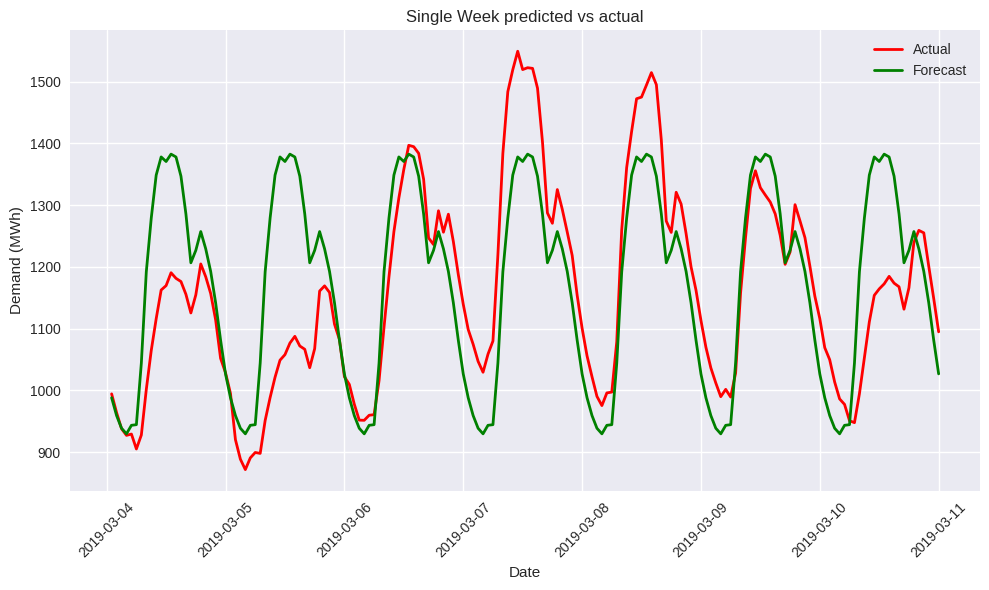
\includegraphics[width=\linewidth]{Chapters/images/results/ES_predicted_vs_actual}
	\caption{The ES predicted results against the actual demand in a week}
	\label{fig:espredictedvsactual}
\end{minipage}
\hfill
% Second figure
\begin{minipage}[b]{0.45\linewidth}
	\centering
	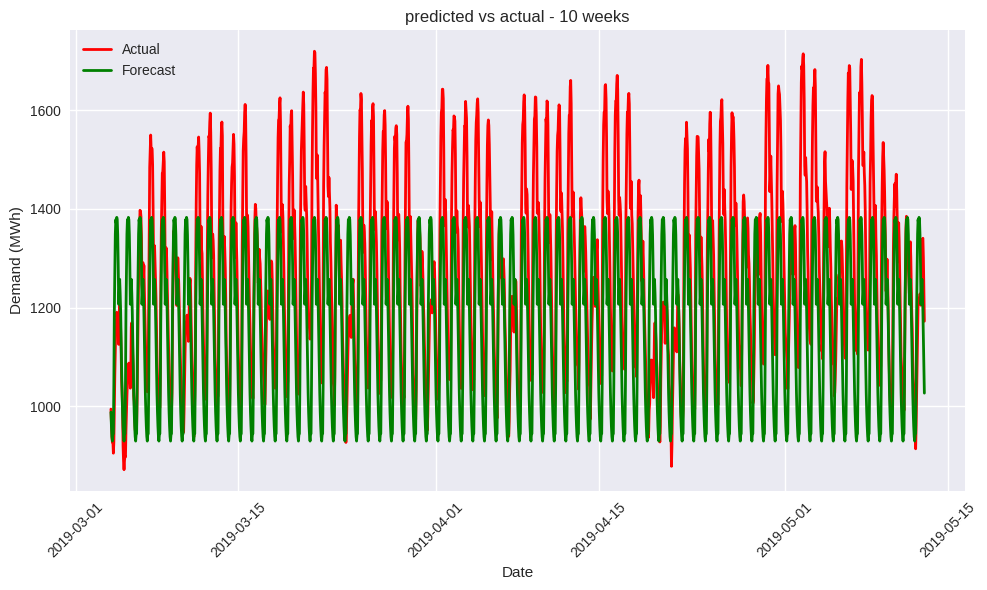
\includegraphics[width=\linewidth]{Chapters/images/results/ES_predicted_vs_actual_10weeks}
	\caption{ES model predicted vs actual load demand over 10 weeks}
	\label{fig:espredictedvsactual10weeks}
	
\end{minipage}
\end{figure}
 Figures \ref{fig:espredictedvsactual} and \ref{fig:espredictedvsactual10weeks} compare the predicted and actual load values. Figure \ref{fig:espredictedvsactual} illustrates the model’s ability to capture the training data patterns; however, it shows limited responsiveness to changing demand features. Figure \ref{fig:espredictedvsactual10weeks} highlights the model’s performance over a longer period, indicating limited generalization, which is consistent with the known limitation of ES models when handling nonlinear and complex time series data.
 
 \subsection{XGBoost Model Results}
 
 The XGBoost model produces an MAPE of 1.598\% and a $R^2$ value of 0.979. This model gradient boosting method enables it to minimize errors on every epoch. This enables it to have a minimized output if test dataset does not significantly change from the training data. The XGBoost models also benefited from the data preprocessing as shown in table \ref{tab:xgboost_comparison} which shows an increased performance with the addition of lag features to the input dataset.
 \begin{table}[h!]
 	\centering
 	\small
 	\caption{Comparison of XGBoost Results with Different Data Processing Techniques}
 		
 	\resizebox{\textwidth}{!}{%
 	\begin{tabular}{lcccc}
 		\hline
 		\textbf{Metric} & \textbf{No Data Processing} & \textbf{Cyclical Encoding (CE)} & \textbf{Only Lag Features} & \textbf{Lag + CE} \\
 		\hline
 		MSE(Mwh)   & 20358  & 12861  & 1519   & 873   \\
 		RMSE(Mwh)  & 143.00 & 113.40 & 38.97  & 29.55 \\
 		MAE(Mwh)   & 115.27 & 91.57  & 27.15  & 18.58 \\
 		MAPE (\%) & 9.46   & 7.65   & 2.34   & 1.64  \\
 		\hline
 	\end{tabular}
 }
 	\label{tab:xgboost_comparison}
 \end{table}
 The models performance is also shown in figure \ref{fig:xgboostoutput}.
 \begin{figure}[h!]
 	\centering
 	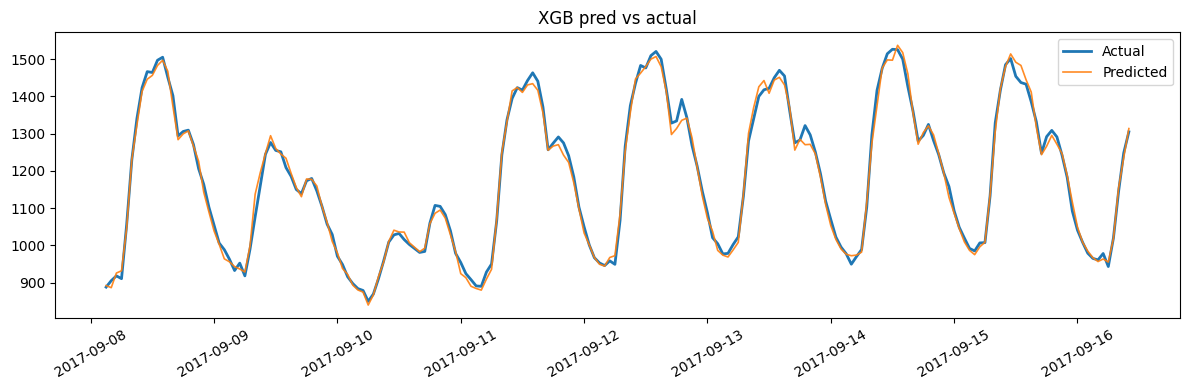
\includegraphics[width=0.75\linewidth]{Chapters/images/results/xgboost_output}
 	\caption{Comparison of XGBoost with the actual load}
 	\label{fig:xgboostoutput}
 \end{figure}
 The model traces the 

\subsection{LSTM model results}
The LSTM model performed better than the ES model producing an MAPE value of 2.82\% and an MAE of 33.48 Mwh.  Table \ref{tab:lstm_performance} contains of the results produced by the LSTM model.
\begin{table}[h]
	\centering
	
	\begin{tabular}{lc}
		\hline
		\textbf{Metric} & \textbf{Value} \\
		\hline
		Mean Squared Error (MSE) & 2319 \\
		Root Mean Squared Error (RMSE) &48.016 \\
		Mean Absolute Error (MAE) & 33.48 \\
		Coefficient of Determination ($R^2$) & 0.933 \\
		Mean Absolute Percentage Error (MAPE) & 2.82\% \\
		\hline
	\end{tabular}
	\caption{LSTM Model Performance Metrics}
	\label{tab:lstm_performance}
\end{table}
 The low MSE and RMSE values indicate that this model has a better fit. The $R^2$ score of 0.933 reflects a robust generalization and the model loss curves in figure \ref{fig:lstmmodel-loss} further show that the model is learning and generalizing properly the the losses settle without fluctuating. 
 \begin{figure}[h]
 	\centering
 	\includegraphics[width=0.9\linewidth]{"Chapters/images/results/lstm_model loss"}
 	\caption{The LSTM model loss during training and validation}
 	\label{fig:lstmmodel-loss}
 \end{figure}
 Figure \ref{fig:lstmpredictedvsactual} shows the comparison of the predicted versus the actual load demand over a period of one week. In this Image it is clear that the model is capable of tracking the actual load very closely.
 \begin{figure}[h]
 	\centering
 	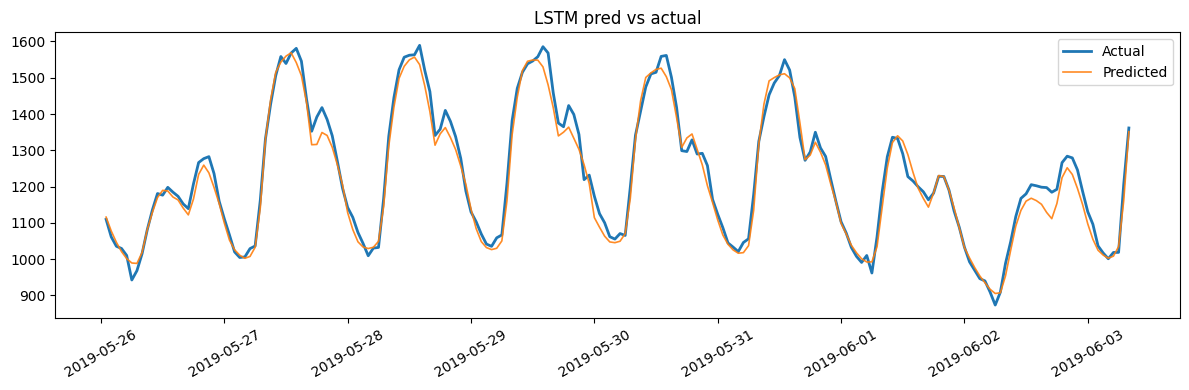
\includegraphics[width=0.5\linewidth]{Chapters/images/results/lstm_predicted_vs_actual}
 	\caption{Comparison of the predicted LSTM output vs the actual demand}
 	\label{fig:lstmpredictedvsactual}
 \end{figure}
 
 
 \subsection{DBN Model results \label{sec:dbn results}}
 The DBN model produced an impressive MAPE value of 2.13\% and an $R^2$ value of 0.966. The $R^2$ value did raise overfitting suspicions as it very high. To ensure that the model is not overfitting the train and test results were compared for the model.
 \begin{table}[h!]
 	\centering
 	\caption{Training and Testing Performance of the DBN Model}
 	\label{tab:dbn_performance}
 	\begin{tabular}{lccc}
 		\hline
 		\textbf{Metric} & \textbf{Train} & \textbf{Test} & \textbf{Difference} \\ \hline
 		MAPE (\%) & 1.6432 & 2.1264 & +0.4832 \\
 		MAE (Mwh) & 18.6358 & 26.3929 & +7.7571 \\
 		RMSE (Mwh) & 25.8889 & 34.7456 & +8.8567 \\
 		R$^2$ & 0.9819 & 0.9655 & -0.0164 \\
 		MSE & 670.23 & 1160.3 & +490.03 \\ \hline
 	\end{tabular}
 \end{table}
  Table \ref{tab:dbn_performance} shows a slightly higher MAE which is expected for non seen data in the test case. The MAPE, RMSE and MSE also show an acceptable increase that represents a normal generalization in the model. The -0.016 drop in the $R^2$ value is minimal meaning that the model has not memorized the training data supporting that the model is not overfitting.
  \begin{figure}[h!]
  	\centering
  	\begin{minipage}[b]{0.45\linewidth}
  		\centering
  		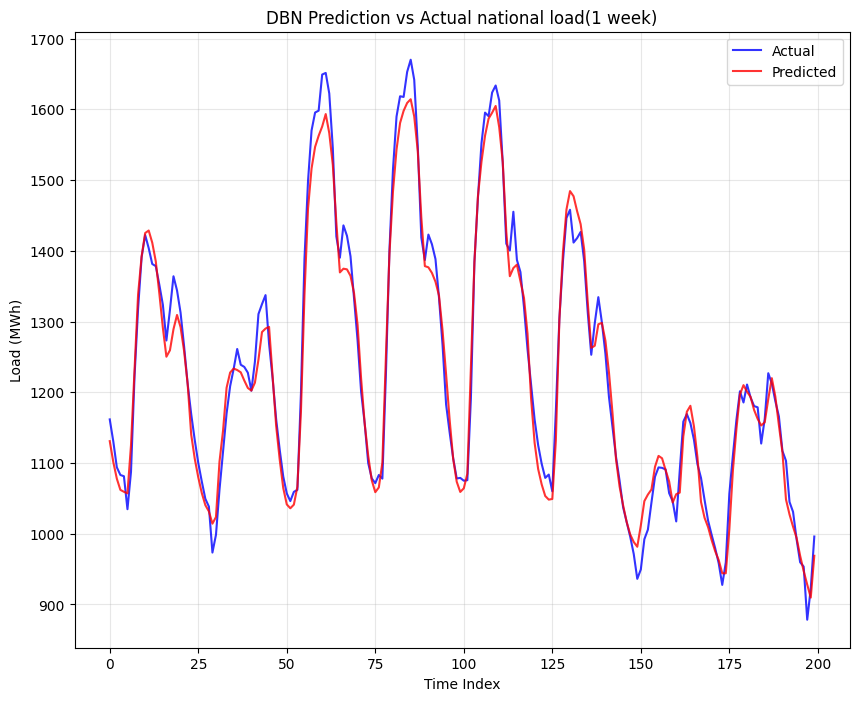
\includegraphics[width=\linewidth]{Chapters/images/results/DBN_predicted_vs_actual}
  		\caption{Predicted vs Actual load over a 1 week period of DBN}
  		\label{fig:dbnpredictedvsactual}
  	\end{minipage}
  	\hfill
  	\begin{minipage}[b]{0.45\linewidth}
  		\centering
  		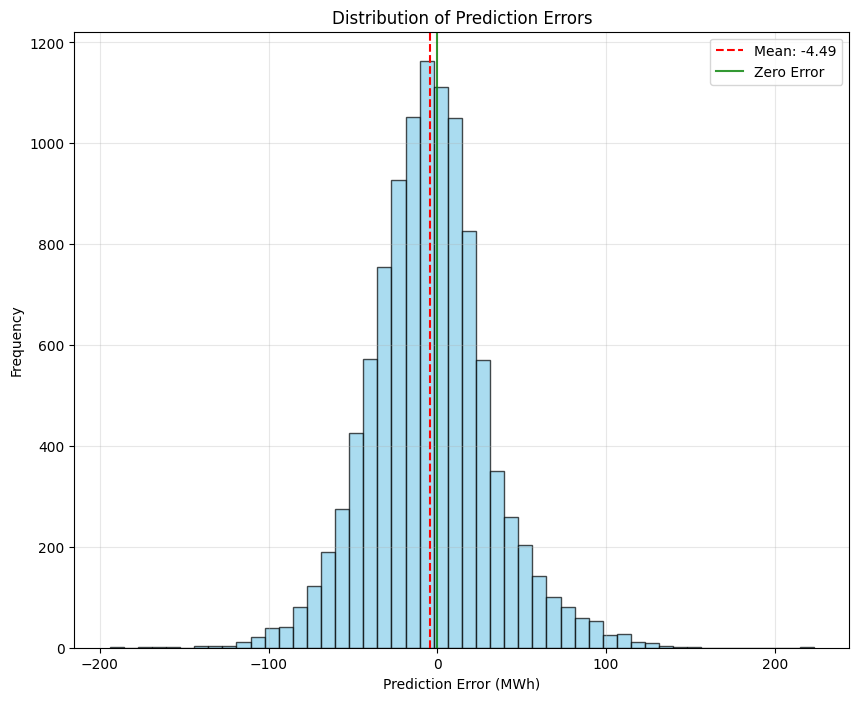
\includegraphics[width=\linewidth]{Chapters/images/results/dbn_error_distribution}
  		\caption{Distribution of prediction errors for the DBN model}
  		\label{fig:dbnerrordistribution}
  	\end{minipage}
  	
  \end{figure}
  
  Figure \ref{fig:dbnpredictedvsactual} illustrates how the predicted load closely follows the actual load over a one-week period. The model’s errors are minimal, as highlighted in Figure \ref{fig:dbnerrordistribution}, which shows the distribution of prediction errors across all test cases. The error distribution approximates a normal distribution, with the majority of errors clustered near zero, indicating strong predictive performance.   
  \begin{figure}[h!]
  	\centering
  	\includegraphics[width=0.4\linewidth]{"Chapters/images/results/dbn_validation loss"}
  	\caption{DBN model loss during training and validation}
  	\label{fig:dbnvalidation-loss}
  \end{figure}
  
 
 
 \subsection{CNN model results}
 
 The CNN model produced a Test MAPE of 2.89\% however similar to the DBN values, with an $R^2$ value of 0.93. Table \ref{tab:cnn_performance_diff} contains the test and train results of the model. The comparison is meant to show if there was a possibility of an overfitting of the data.
 \begin{table}[h!]
 	\small
 	\centering
 	\caption{Performance Metrics of the CNN Model}
 	\label{tab:cnn_performance_diff}
 	\begin{tabular}{lccc}
 		\hline
 		\textbf{Metric} & \textbf{Training} & \textbf{Test} & \textbf{Difference} \\
 		\hline
 		MAPE (\%) & 1.4700 & 2.887 & +1.4170 \\
 		MAE (Mwh) & 16.713 & 33.976& +16.364 \\
 		RMSE (Mwh) & 25.282 & 33.976 & +8.6946 \\
 		R$^2$ & 0.9827 & 0.9250 & -0.0578 \\
 		MSE & 639.17 & 2564.2 & +1925.0 \\
 		\hline
 	\end{tabular}
 \end{table}
Similar to the results obtained for the DBN model (Section \ref{sec:dbn results}), the high $R^2$ values observed do not imply overfitting. The elevated $R^2$ can be attributed to the inclusion of additional engineered features generated during data preprocessing and feature engineering. As no discussed by Plevris et al. \cite{plevris2022investigation}, the $R^2$ value tends to increase with more features, even when some of these features do not directly correlate with the  output. Figure \ref{fig:cnnmodelloss} shows how the train and value loss change over the epochs. The image shows a smooth decline in the train loss, however the validation loss has a fluctuating loss that does not converge.
Figure \ref{fig:cnnpredictionvsactual} shows the prediction vs the actual output of the CNN model. The predicted load closely follows the actual load.
\begin{figure}[h!]
	\centering
	\begin{minipage}[b]{0.46\linewidth}
	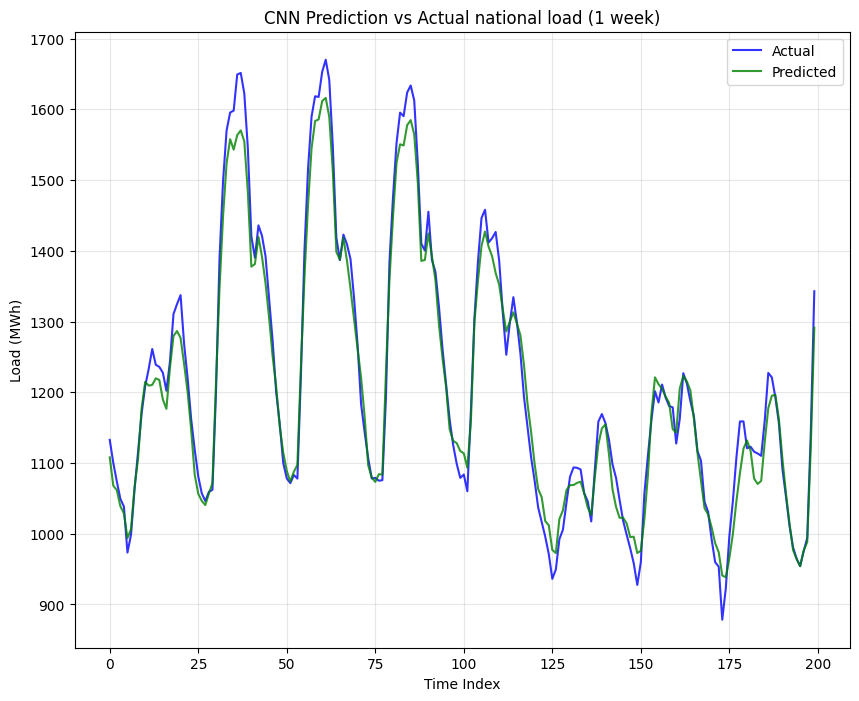
\includegraphics[width=\linewidth]{Chapters/images/results/cnn_predictionvsactual}
	\caption{The predicted and actual loading from the CNN model}
	\label{fig:cnnpredictionvsactual}
	\end{minipage}
	\begin{minipage}[b]{0.46\linewidth}
	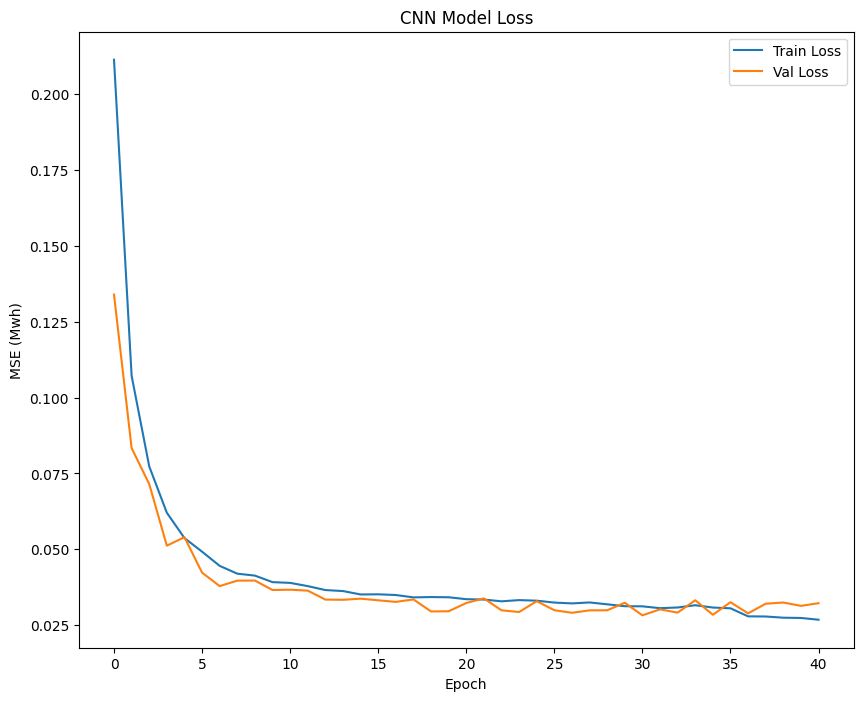
\includegraphics[width=\linewidth]{Chapters/images/results/CNN_model_loss}
	\caption{The CNN model validation and test loss against the epochs}
	\label{fig:cnnmodelloss}
	\end{minipage}
\end{figure}

\subsection{Hybrid Model Results: CNN-LSTM}
 The hybrid model produced an MAPE of 2.9\% and a MAE of 34.63Mwh. The table \ref{tab:cnn-lstm-results} shows the results produced by the hybrid model.
  \begin{table}[h]
 	\centering
 	\caption{Performance Metrics of the CNN Model}
 	\label{tab:cnn-lstm-results}
 	\begin{tabular}{lccc}
 		\hline
 		\textbf{Metric} & \textbf{Test} \\
 		\hline
 		MAPE (\%) &  2.902 \\
 		MAE (Mwh) &   34.63  \\
 		RMSE (Mwh) &  48.60  \\
 		R$^2$ &  0.929  \\
 		MSE & 2464  \\
 		\hline
 	\end{tabular}
 \end{table}
 \begin{figure}[h]
 	\centering
 	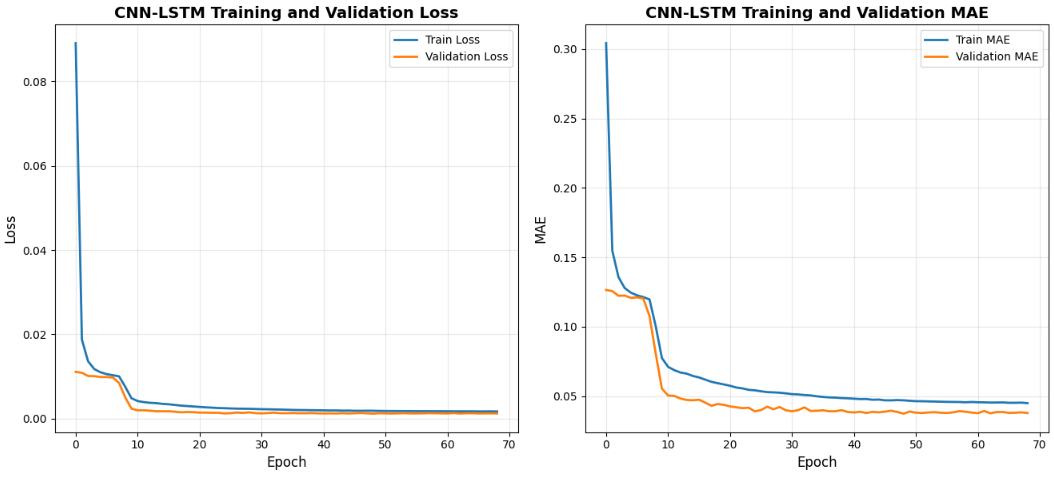
\includegraphics[width=0.9\linewidth,height=0.3\textwidth]{Chapters/images/results/CNN-LSTM-MODEL-LOSS}
 	\caption{Model train and validation loss over 69 epochs.}
 	\label{fig:cnn-lstm-model-loss}
 \end{figure}
Figure \ref{fig:cnn-lstm-model-loss} shows a settling in the training and validation loss. The MAE loss it also below the train MAE which shows normalcy in the training process. Figure \ref{fig:cnnlstmpredictionvsactual} shows the prediction and actual load over a period of a week. The plot shows close tracing however this does not provide the full figure of the performance of the model.
 \begin{figure}[h]
 	\centering
 	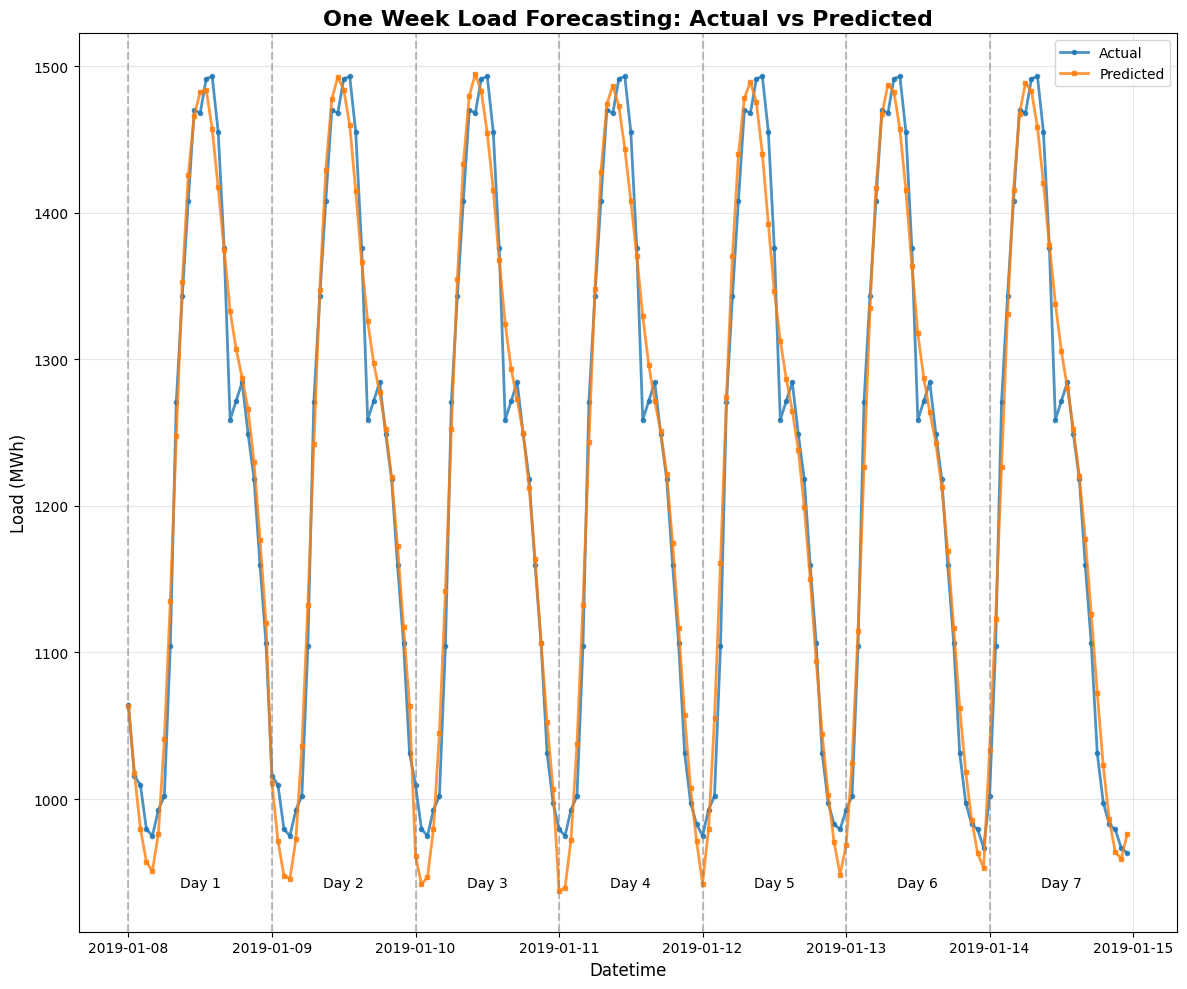
\includegraphics[width=0.9\linewidth,height=0.38\textwidth]{Chapters/images/results/cnn_lstm_prediction_vs_actual}
 	\caption{comparison of predicted vs actual load in a CNN-LSTM model}
 	\label{fig:cnnlstmpredictionvsactual}
 \end{figure}
 
 In order to show the complete performance of the model, figure \ref{fig:cnnlstmpredictionvsactualfull} shows the performance of the model across all the samples. This shows that though the model is capable of predicting in most cases there is a period of low demand that the model fails to generalize well. This may be due to a phenomenon where the demand dropped but the features used in the model were consistent with the training data.
 \begin{figure}[h]
 	\centering
 	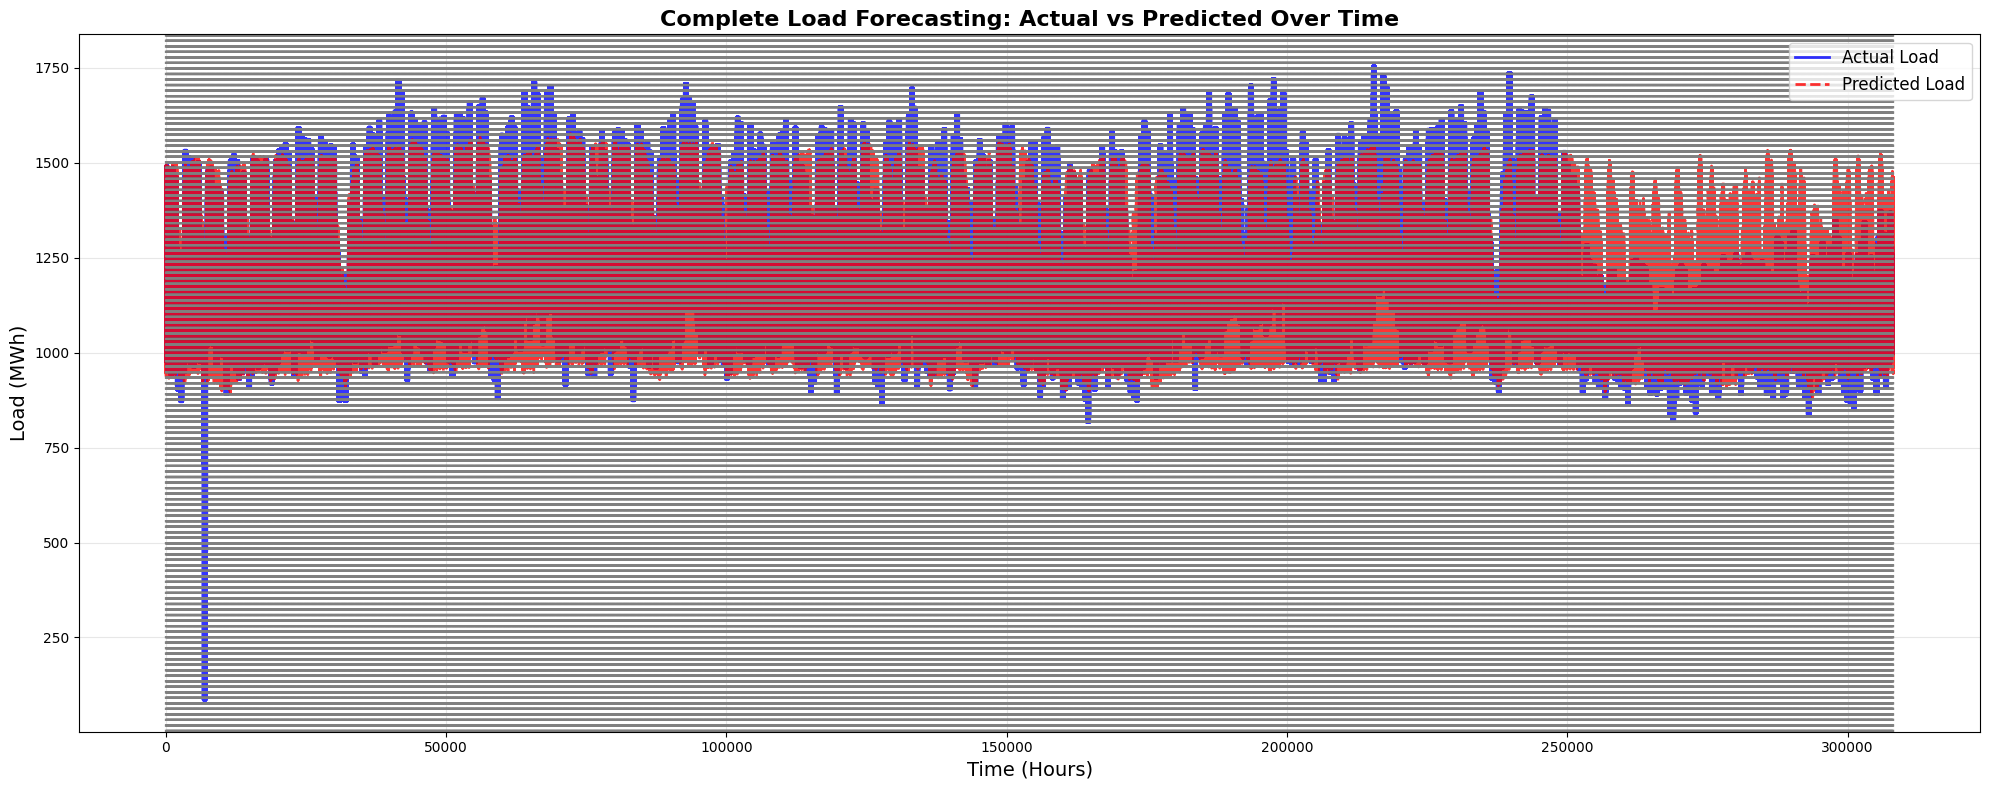
\includegraphics[width=0.9\linewidth,height=0.3\textwidth]{Chapters/images/results/cnn_lstm_prediction_vs_actual_full}
 	\caption{The complete comparison of the CNN-LSTMs predicted vs actual demand}
 	\label{fig:cnnlstmpredictionvsactualfull}
 \end{figure}
 
 
 \section{Comparative Results}
 
The six models tested in this research were trained and tested on data with an 80/20 train-test split. The validation was set to a 20\% of the testing data. The performance metrics of the models have been captured in Table \ref{tab:model-performance}. The table contains the MAPE values which show the XGBoost model performing the best amongst all the models. The ES model however had the highest MAPE representing a lack of generalization of the model, this is also further backed by its $r^2$ value.

 
 \begin{table}[htbp]
 	\centering
 	\small
 	\caption{Performance comparison of forecasting models}
 	\label{tab:model-performance}
 	
 	\resizebox{\textwidth}{!}{%
 	\begin{tabular}{lrrrrr}
 		\hline
 		\textbf{Model} & \textbf{MSE (Mwh)} & \textbf{MAE (MwH)} & \textbf{MAPE (\%)} & \textbf{RMSE (Mwh)} & \textbf{R\textsuperscript{2}} \\
 		\hline
 		Exponential Smoothing & 20,118 & 118.14 & 9.57 & 141.84 & 0.5241 \\
 		XGBoost               & 719.58 & 19.06  & 1.598 & 26.82  & 0.979  \\
 		DBN                   & 1,160  & 24.87  & 2.1   & 34.06  & 0.966  \\
 		CNN                   & 2,564  & 33.97  & 2.887 & 50.64  & 0.925  \\
 		LSTM                  & 2,319  & 33.48  & 2.82  & 48.016 & 0.933  \\
 		CNN-LSTM              & 2,464  & 34.63  & 2.902 & 48.64  & 0.929  \\
 		\hline
 	\end{tabular}}
 \end{table}
 To show the comparison of the comparison metrics of the model, the bar graphs \ref{fig:rmsecomparison}, \ref{fig:maecomparison} and \ref{fig:mapecomparison1}. These graphs help paint a clearer picture of the comparison between the models.
 Figure \ref{fig:rmsecomparison} shows that the ES model having the largest RMSE value while the XGBoost followed by the DBN Model. This is the same representation of the metrics in figure \ref{fig:maecomparison} and \ref{fig:mapecomparison1}.
 
 \begin{figure}[h]
 	\centering
 	\begin{minipage}[b]{0.325\linewidth}
 		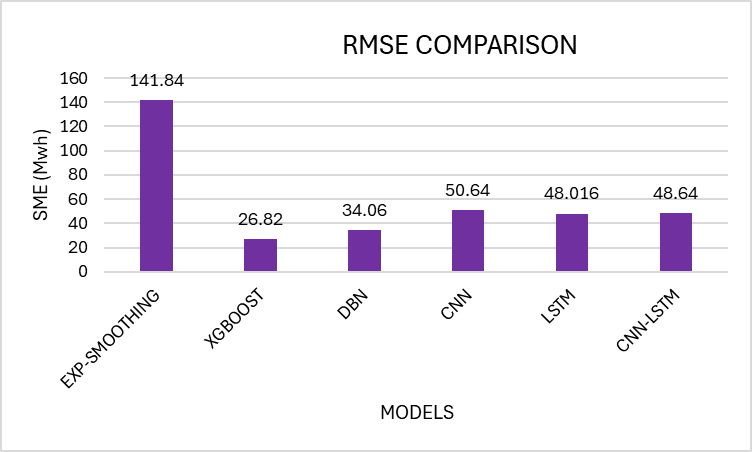
\includegraphics[width=\linewidth]{Chapters/images/results/RMSE_COMPARISON}
 		\caption{RMSE Comparison}
 		\label{fig:rmsecomparison}
 	\end{minipage}
 	\begin{minipage}[b]{0.325\linewidth}
 		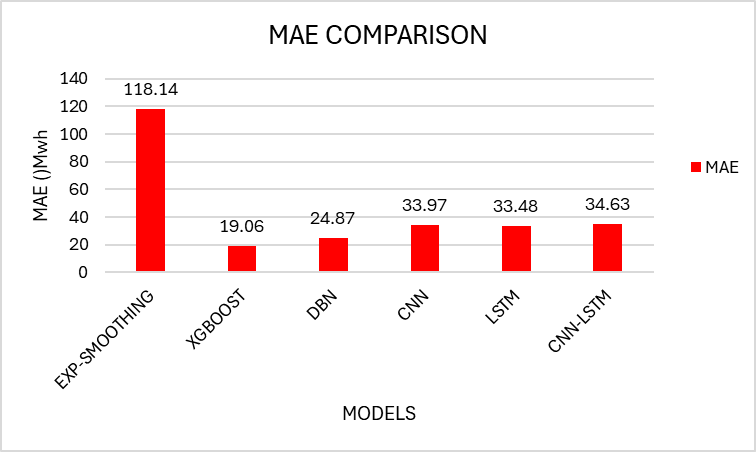
\includegraphics[width=\linewidth]{Chapters/images/results/MAE_COMPARISON}
 		\caption{MAE Comparison}
 		\label{fig:maecomparison}
 	\end{minipage}
 	\begin{minipage}[b]{0.325\linewidth}
 		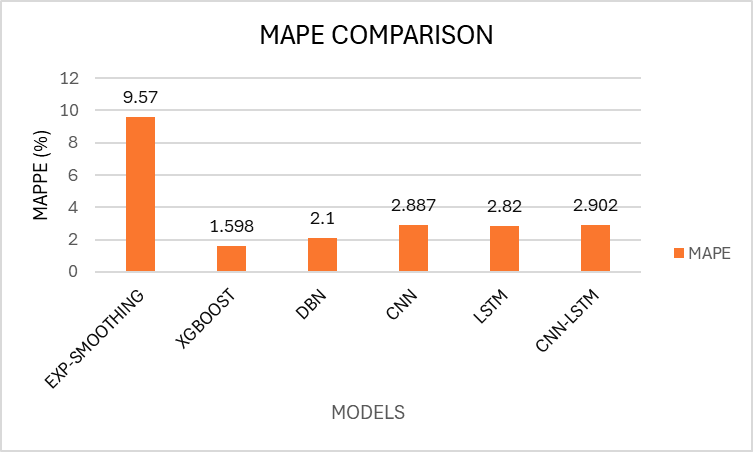
\includegraphics[width=\linewidth]{Chapters/images/results/MAPE_COMPARISON1}
 		\caption{MAPE Comparison}
 		\label{fig:mapecomparison1}
 	\end{minipage}
 \end{figure}
 
 Table \ref{tab:model-performance} and the images showing the performance of the models numerically. The images below compare how well the model traces the actual load data in real time. 


 \begin{figure}[h!]
 	\centering
 	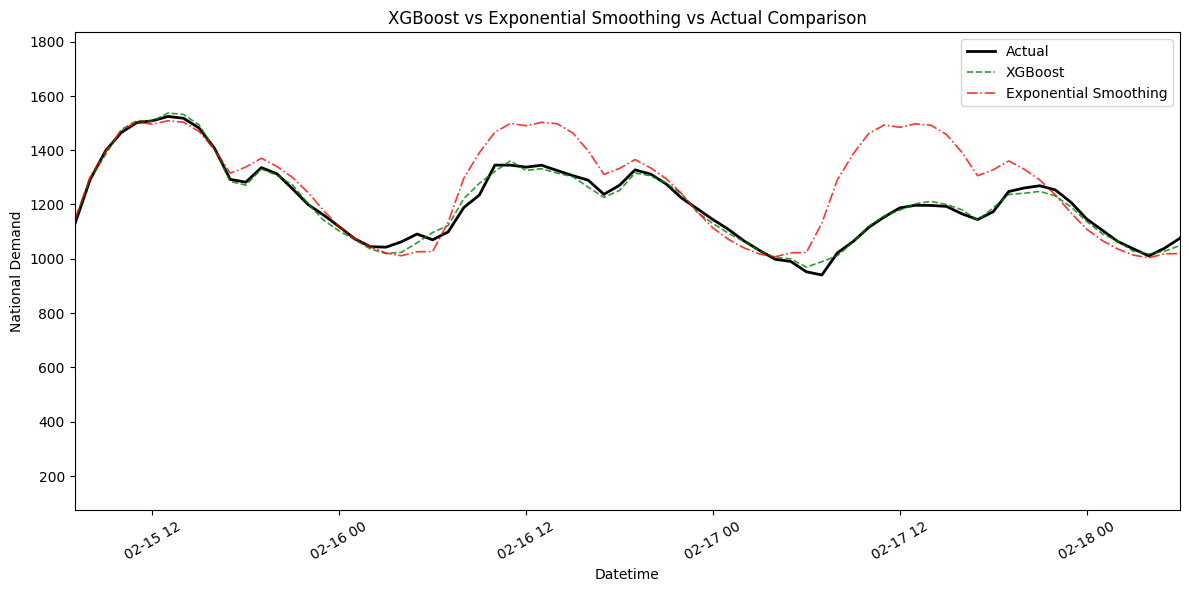
\includegraphics[width=0.75\linewidth]{Chapters/images/results/xgboost_vs_expsmoothing}
 	\caption{XGBoost vs ES and the actual load}
 	\label{fig:xgboostvsexpsmoothing}
 \end{figure}
 
 Figure \ref{fig:xgboostvsexpsmoothing} shows the comparison of the xgboost, ES model and the actual load data over a period of three days. The result is showing a very close tracing the actual load. On the other hand the ES models fails to set itself to the values on the peaks. this results in the ES model having higher peaks than the actual the load data.
 
 \begin{figure}[h!]
 	\centering
 	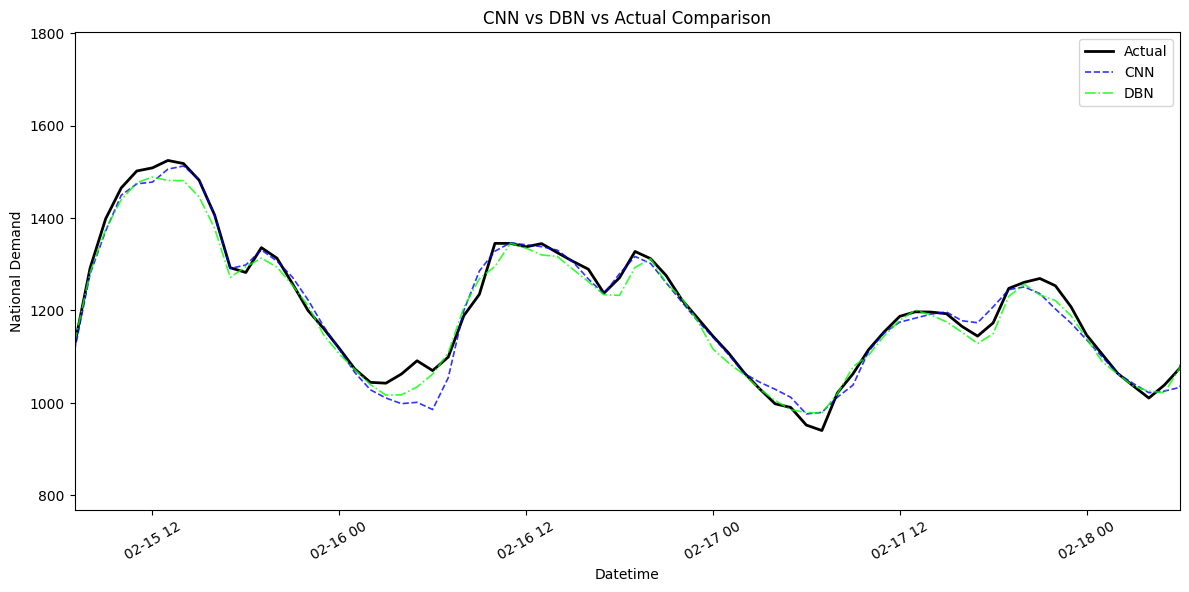
\includegraphics[width=0.75\linewidth]{Chapters/images/results/cnn_vs_dbn_actual}
 	\caption{DBN compared to CNN}
 	\label{fig:cnnvsdbnactual}
 \end{figure}
 The DBN and CNN have a similar neural network architecture with multilevel features on both models. Their performance was also compared to each other and in figure \ref{fig:cnnvsdbnactual} the models are compared to each other. Table \ref{tab:model-performance} shows the DBN outperforming the CNN on all performance parameters and this is also highlighted in figure \ref{fig:cnnvsdbnactual}. The two models trace the actual load very well however the CNN model fails to trace at certain points on dips. The difference is negligible though as the difference in their MAPE values is 0.7\%.
 \begin{figure}[h!]
 	\centering
 	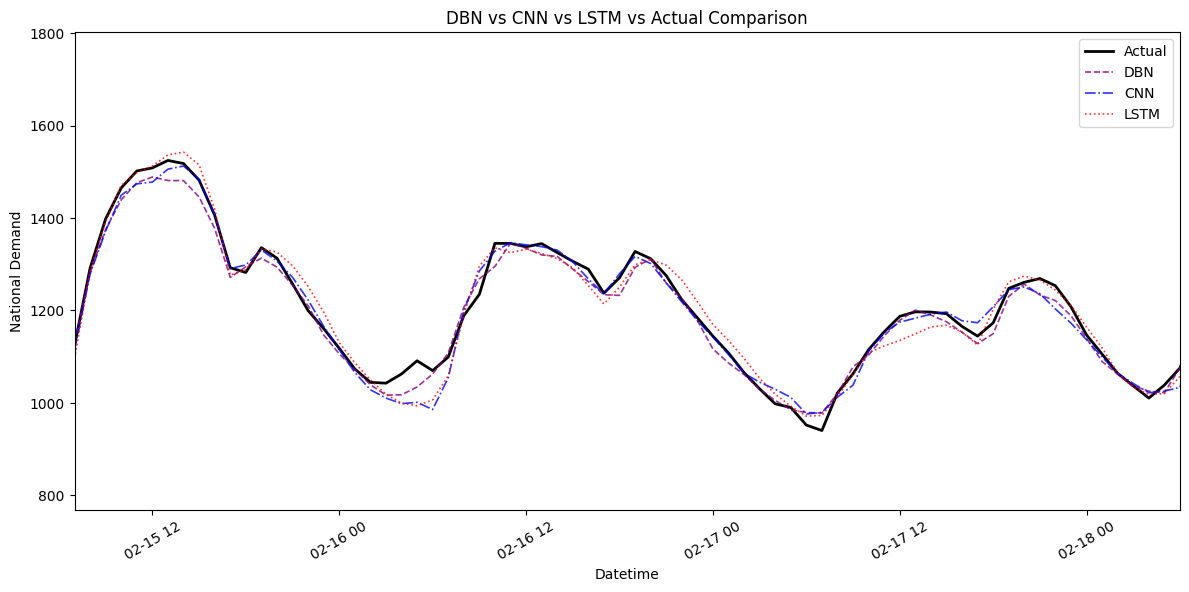
\includegraphics[width=0.75\linewidth]{Chapters/images/results/cnn_vs_dbn_vs_lstm_vs_actual}
 	\caption{DBN, CNN, LSTM and actual compared to each other}
 	\label{fig:cnnvsdbnvslstmvsactual}
 \end{figure}
 
 Further in the comparison of the models in figure \ref{fig:cnnvsdbnvslstmvsactual} compares the Deep learning models usd in the research. The performance metrics shows that the DBN performs best with a MAPE of 2.1\% while LSTM and CNN trail close behind with 2.82\% and 2.89\% respectively. Figure \ref{fig:cnnvsdbnvslstmvsactual} shows the three models tracing the actual load. IT however shows the CNN and LSTM trailing behind on the dips which is expected because of their higher MAPE, MAE and RMSE values.
  \begin{figure}[h!]
 	\centering
 	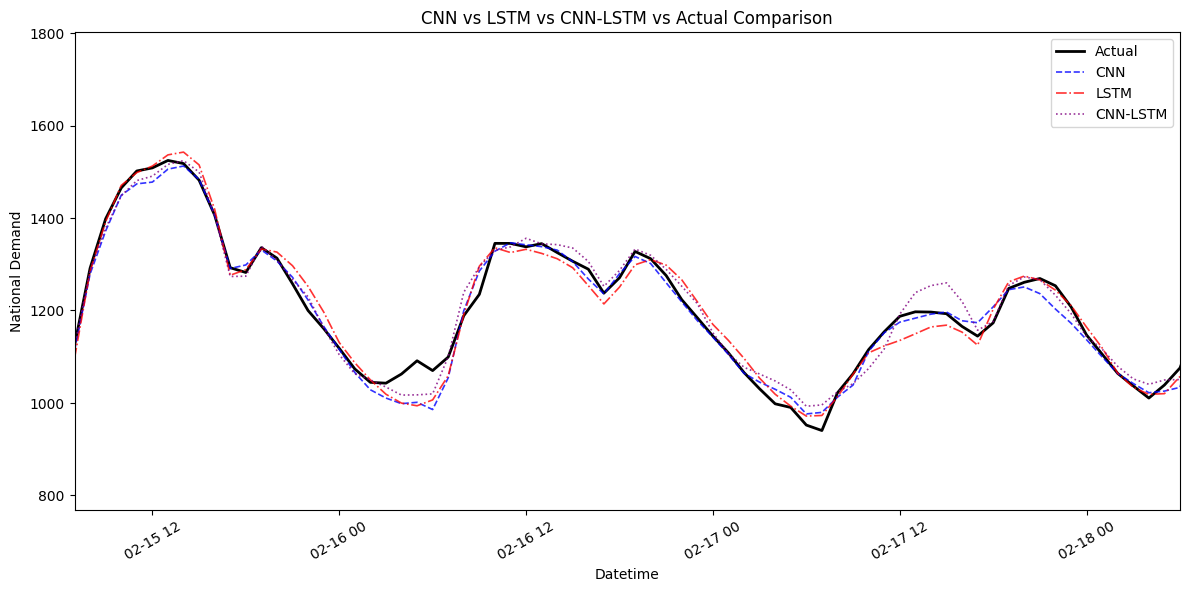
\includegraphics[width=0.75\linewidth]{Chapters/images/results/cnn_vs_lstm_vs_cnn-lstm_vs_actual}
 	\caption{CNN, LSTM, CNN-LSTM compared to each other}
 	\label{fig:cnnvslstmvscnn-lstmvsactual}
 \end{figure}
 
The CNN-LSTM model being a hybrid of the CNN and LSTM model, the performance of the three was also compared. Figure \ref{fig:cnnvslstmvscnn-lstmvsactual} shows the comparison. The hybrid model does not show a very big improvement in the hybrid model, it however shows a mixture of improved performances at different points in the shown tiem with each of the models taking turns at being good. Their values in \ref{tab:model-performance} are also close to each other showing an actual slight decrease in its MAPE with 2.902\% which is 0.1\% higher than the CNN and LSTM models.
 
  
 \begin{figure}[h]
 	\centering
 	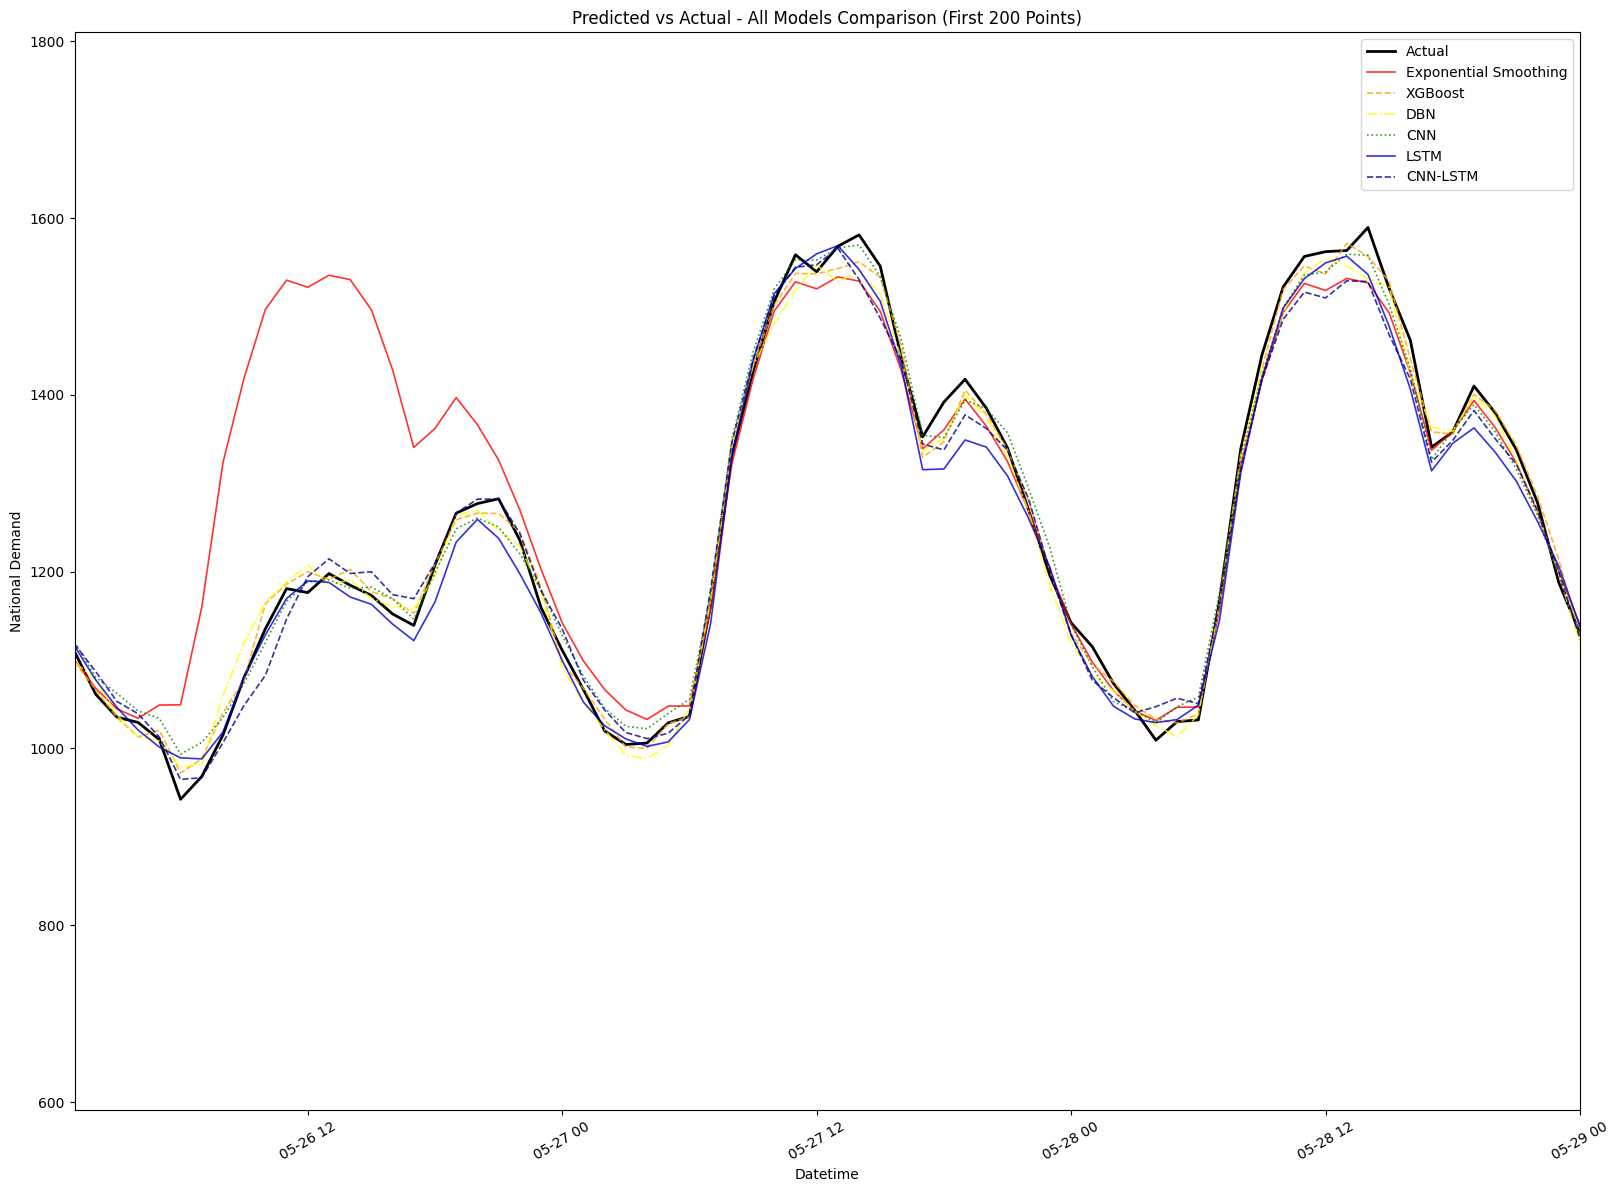
\includegraphics[width=0.8\linewidth]{Chapters/images/results/all_model_comparison}
 	\caption{performance comparison of 6 models}
 	\label{fig:allmodelcomparison}
 \end{figure}
  Finally in figure \ref{fig:allmodelcomparison} we compare the performance of all the models used in the research. Supported by the table of results, \ref{tab:model-performance} the ES model manages to trace really well when load peaks and troughs are in the weekly range, however dues to its generalization once the load data reduces such as on weekends it fails to adjust accordingly causing the high error in the models. All the other models performance can not be conclusive from just looking at the performance curves. However the CNN-LSTM  and CNN models fail to generalize on the peaks and troughs. All models show  great capability in leaning the increases in the data as they trace the actual load with minimum error. The data shown in figure \ref{fig:allmodelcomparison} supports the data that was collected in table \ref{tab:model-performance}.
 